\documentclass{beamer}

\usepackage{kotex}
\usepackage{graphicx}
\usepackage{minted}
\usepackage[export]{adjustbox}

\vfuzz=30pt

%%%%%%%%%%%%%%%%%%%%%
%  Beamer Settings  %
%%%%%%%%%%%%%%%%%%%%%
\usetheme[numbering=fraction]{metropolis}
\usecolortheme{rose}
\useoutertheme[subsection=false]{miniframes}

\setbeamertemplate{itemize item}[square]
\setbeamertemplate{itemize subitem}[triangle]
\setbeamertemplate{itemize subsubitem}[circle]

%%%%%%%%%%%%%%%%%%%
%  Font Settings  %
%%%%%%%%%%%%%%%%%%%
\usepackage[factor=500]{microtype}

\usepackage[mathrm=sym]{unicode-math}

\setmainfont{TeXGyrePagellaX}
\setsansfont{Roboto}[
  BoldFont = *-Medium,
  BoldItalicFont = *-MediumItalic
]
\setmonofont{Inconsolata}

\setmainhangulfont{NanumMyeongjo}
\setsanshangulfont{NanumGothic}[AutoFakeSlant=0.18]

\setmathfont{Fira Math}
\setmathfont{Fira Sans Medium}[range=bfsfup]
\setmathfont{Fira Sans Medium Italic}[range=bfsfit]
\setmathfont{STIX Two Math}[range=cal]

%%%%%%%%%%%%%%%%%%%%%
%  Minted Settings  %
%%%%%%%%%%%%%%%%%%%%%
\renewcommand\theFancyVerbLine{\textsf{\tiny\arabic{FancyVerbLine}}}

\newminted{latex}{
  escapeinside=||,
  autogobble,
  linenos,
  breaklines,
  numbersep=5pt,
  frame=single,
  fontsize=\scriptsize}
\newmintinline[ltxverb]{latex}{}

%%%%%%%%%%%%%%%%%%%%%%%
%  Document Settings  %
%%%%%%%%%%%%%%%%%%%%%%%

\title{%
  {\large memoir와 expl3로 해보는 Book Design}\\
  Page Style
}

\author{이재호}
\institute{memoir 스터디 그룹}
\date{\today}

%%%%%%%%%%%%%%
%  Document  %
%%%%%%%%%%%%%%
\begin{document}

\maketitle

\section{Make Page Style}

\begin{frame}[fragile]{\texttt{\textbackslash make[even|odd][head|foot]}}
  \begin{columns}
    \begin{column}{0.6\textwidth}
      \begin{latexcode}
        \makepagestyle{demo}
        \makeevenhead{demo}{ehl}{ehc}{ehr}
        \makeoddhead{demo}{ohl}{ohc}{ohr}
        \makeevenfoot{demo}{efl}{efc}{efr}
        \makeoddfoot{demo}{ofl}{ofc}{ofr}
      \end{latexcode}
    \end{column}

    \begin{column}{0.4\textwidth}
      \begin{overprint}
        \onslide<1>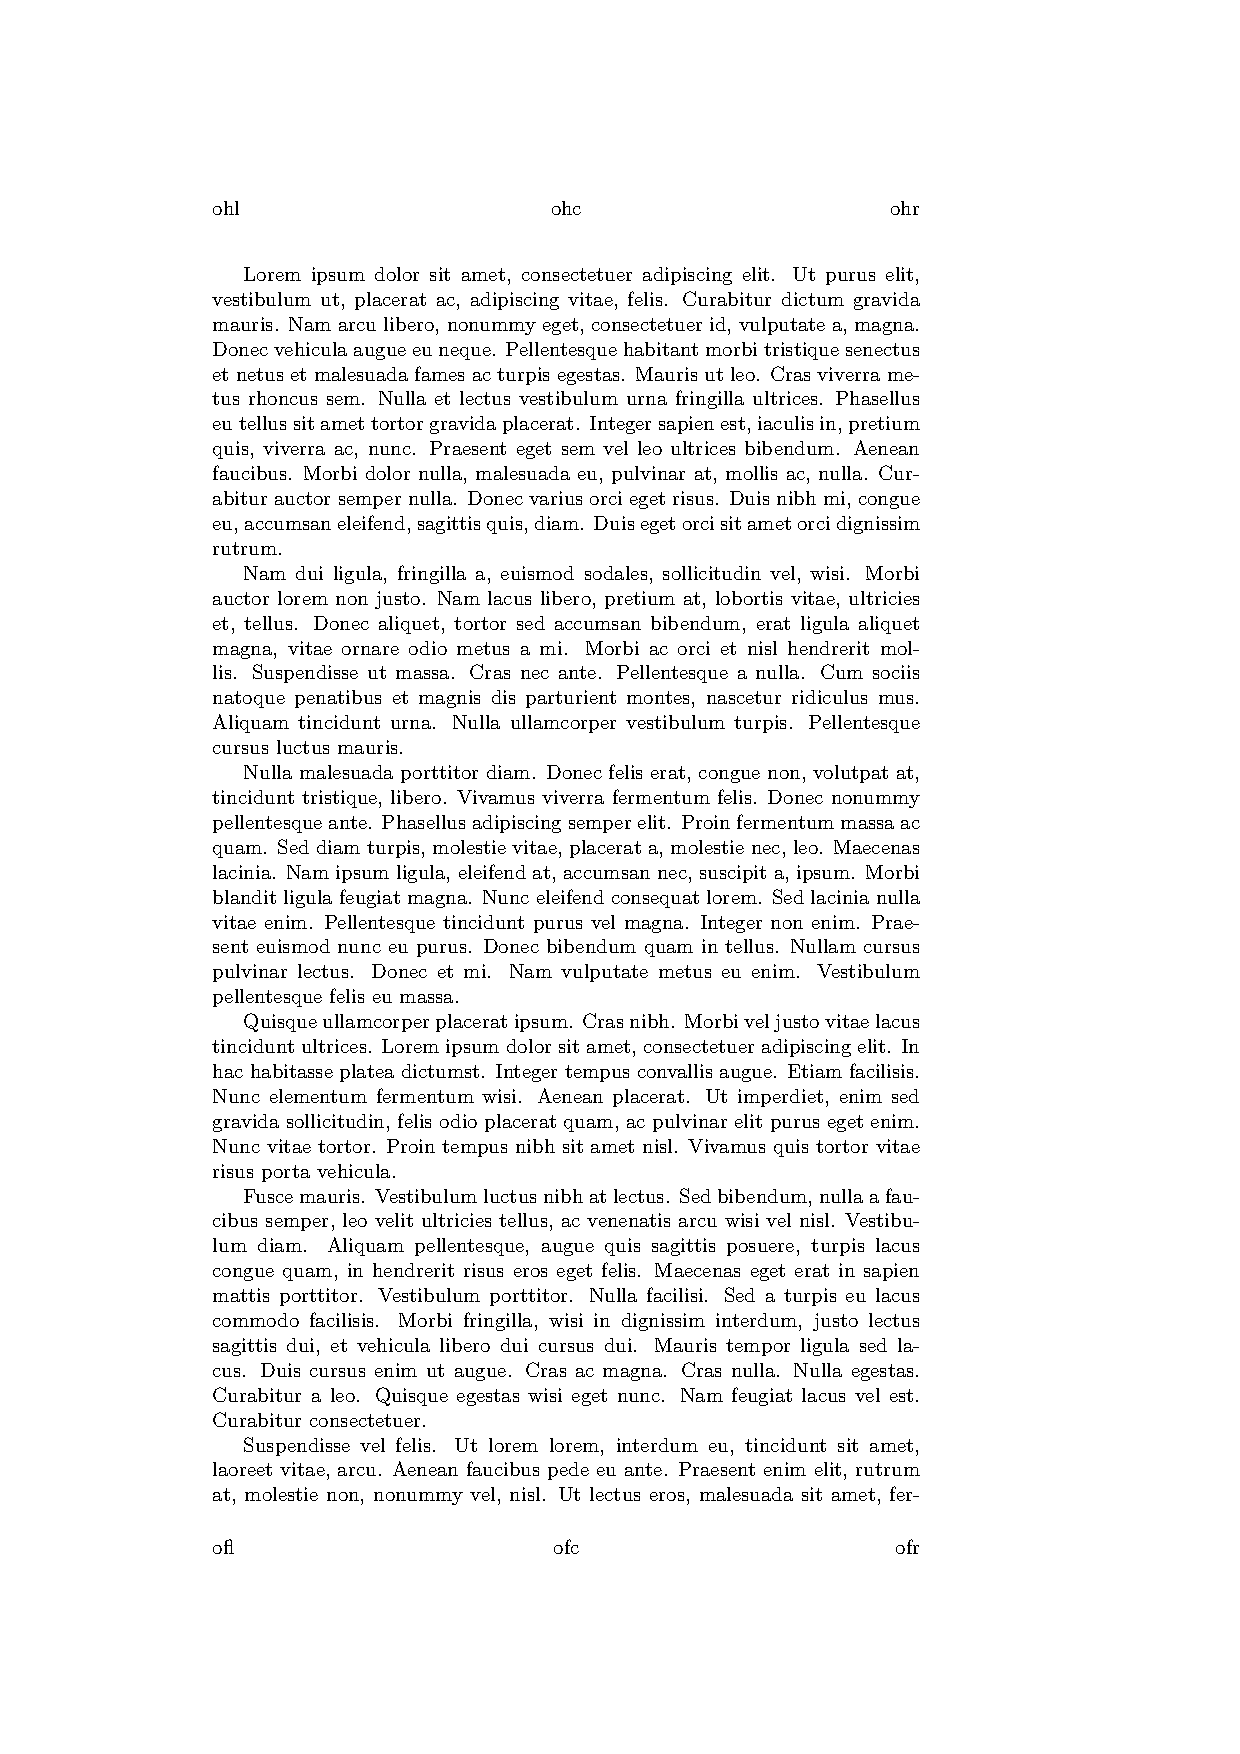
\includegraphics[frame,width=\linewidth]{demo-hf-1}
        \onslide<2>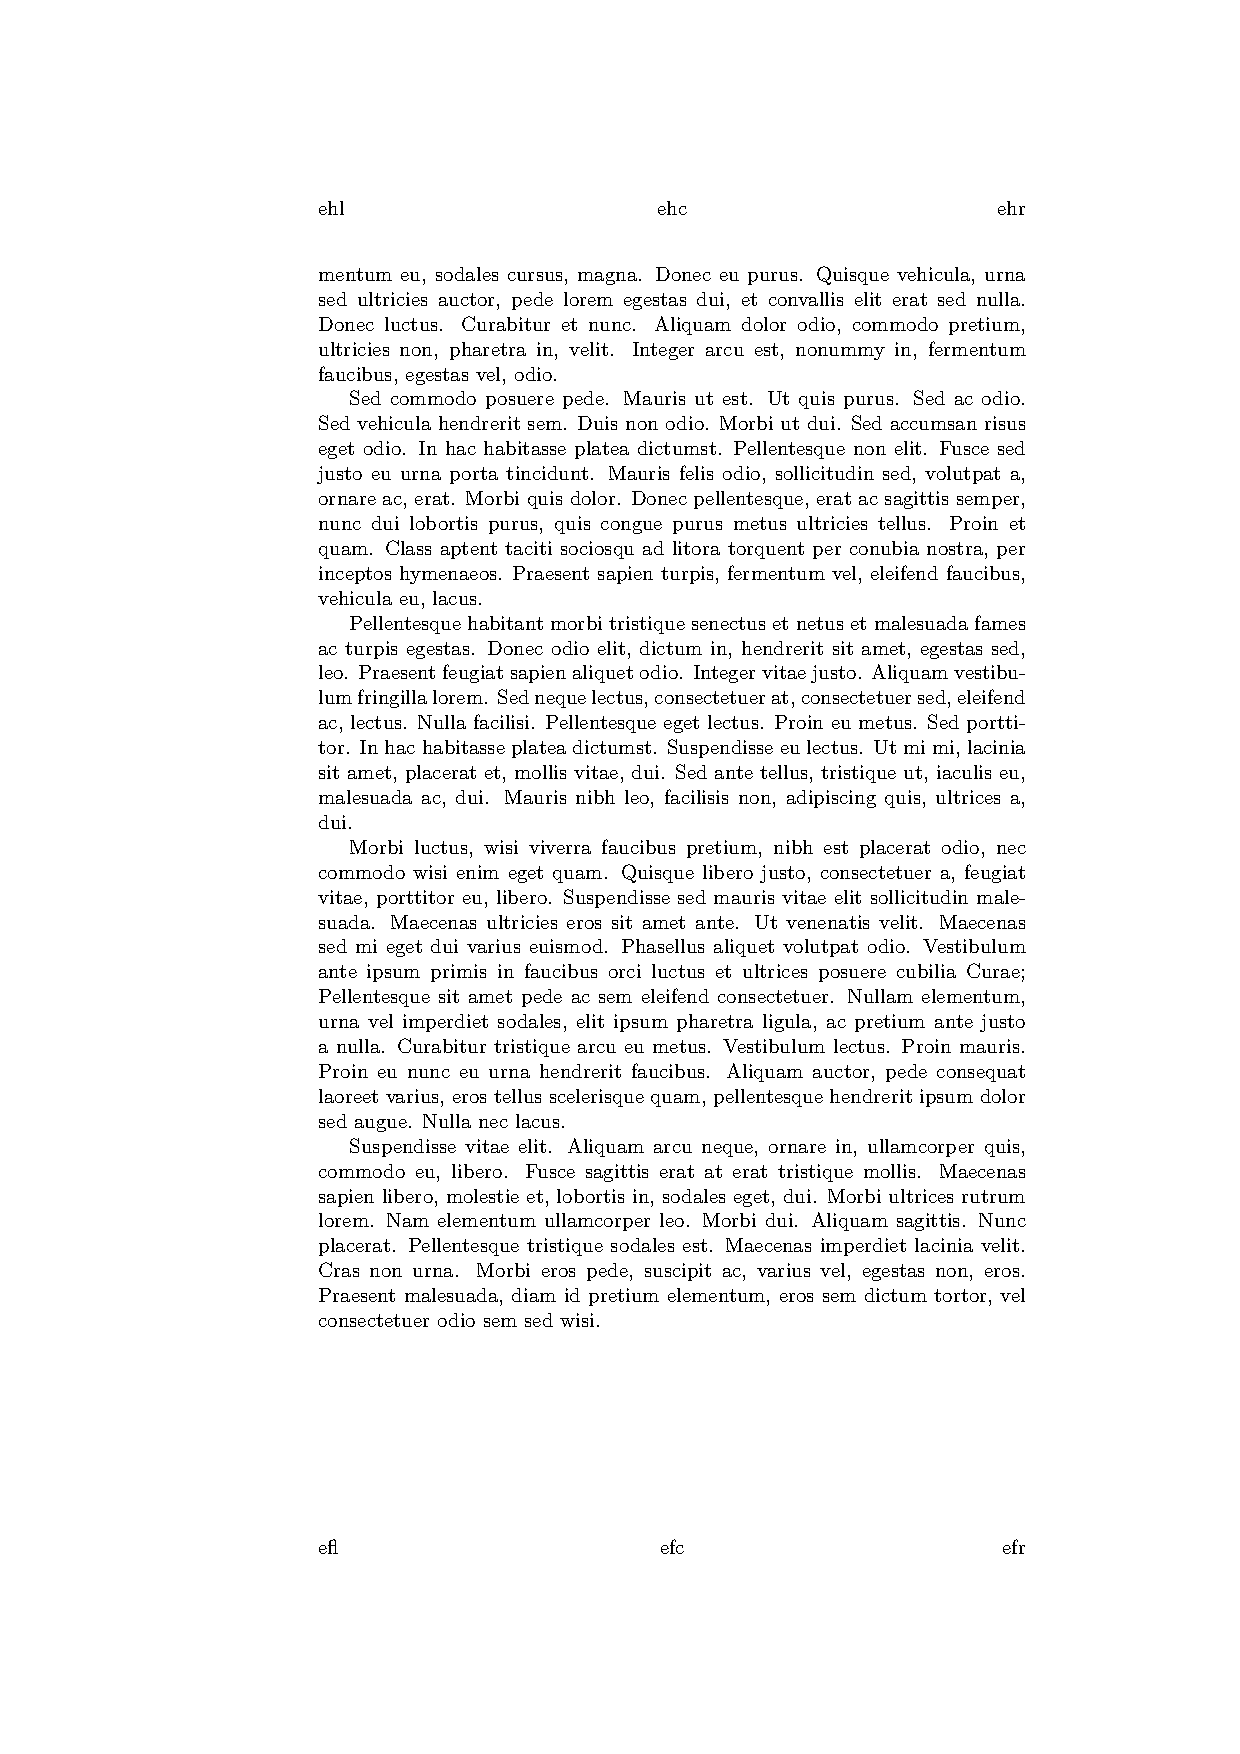
\includegraphics[frame,width=\linewidth]{demo-hf-2}
      \end{overprint}
    \end{column}
  \end{columns}
\end{frame}

\begin{frame}[fragile]{\texttt{moresimple} Page Style}
  \begin{columns}
    \begin{column}{0.6\textwidth}
      \begin{latexcode}
        \makepagestyle{moresimple}
        \makeevenfoot{moresimple}{\thepage}{}{}
        \makeoddfoot{moresimple}{}{}{\thepage}
      \end{latexcode}
    \end{column}

    \begin{column}{0.4\textwidth}
      \begin{overprint}
        \onslide<1>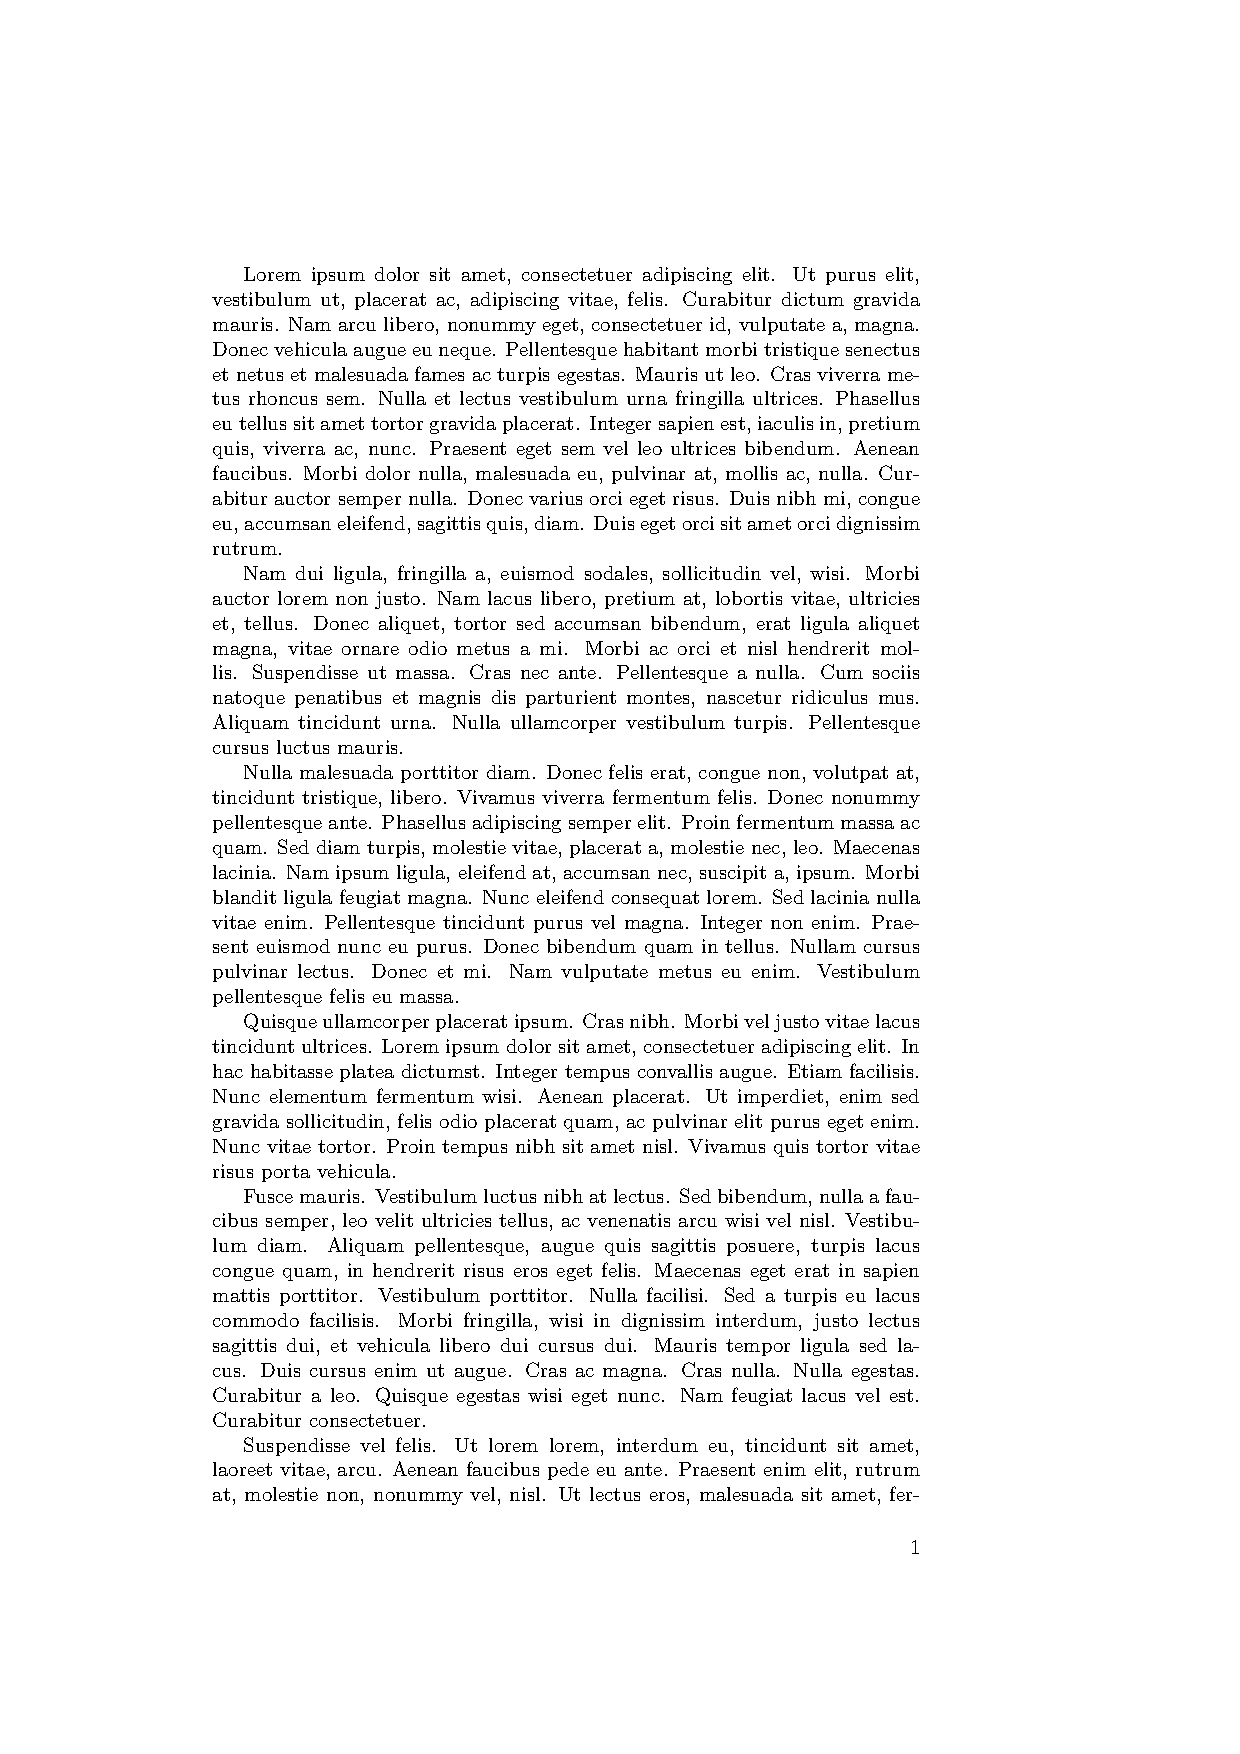
\includegraphics[frame,width=\linewidth]{moresimple-hf-1}
        \onslide<2>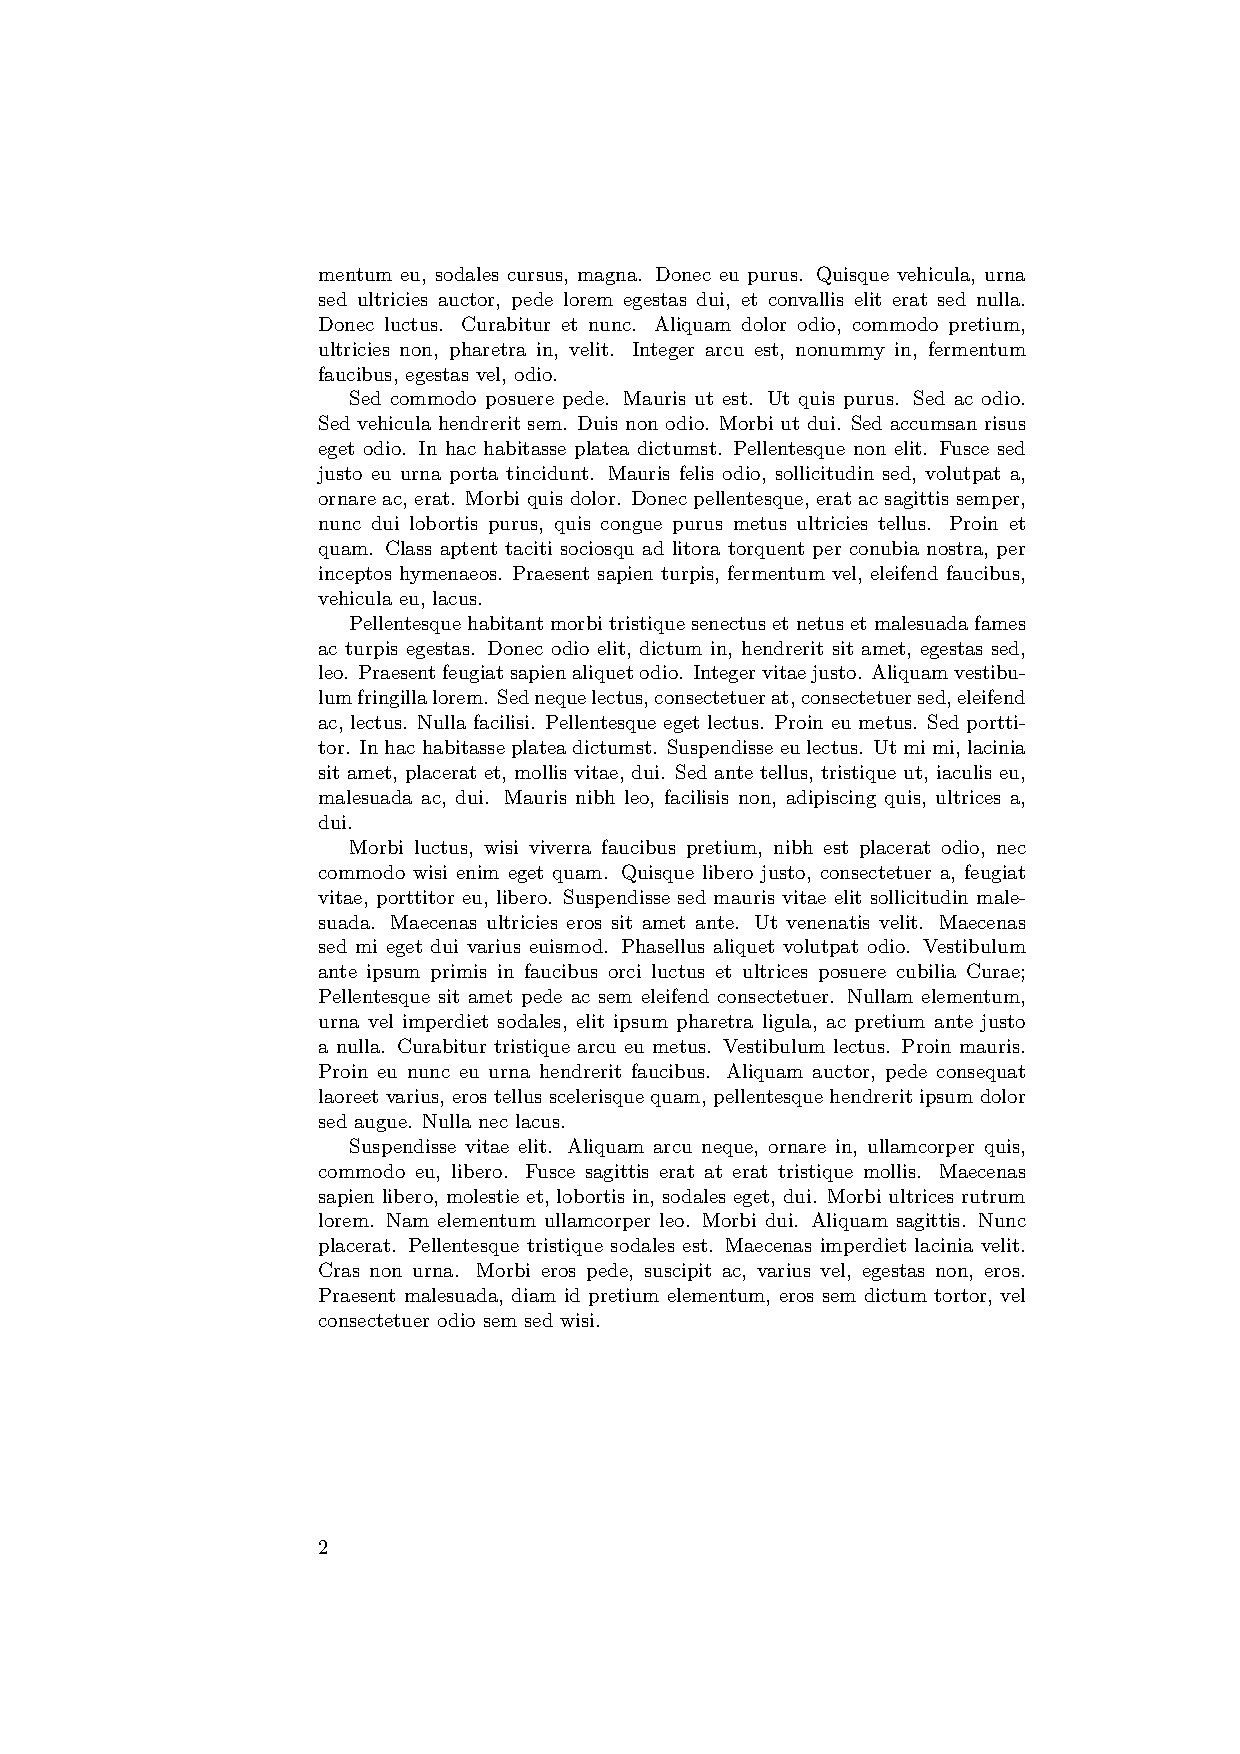
\includegraphics[frame,width=\linewidth]{moresimple-hf-2}
      \end{overprint}
    \end{column}
  \end{columns}
\end{frame}


\section{Rules}

\begin{frame}[fragile]{Rules}
  \begin{columns}
    \begin{column}{0.6\textwidth}
      \begin{latexcode}
        % \usepackage[dvipsnames]{xcolor}
        \makepagestyle{demo}
        \makeheadrule{demo}{\textwidth}{1pt}
        \makefootrule{demo}{\textwidth}{1pt}|\linebreak|{\footruleskip}
        \makeheadfootruleprefix{demo}|\linebreak|{\color{RoyalPurple}}{\color{Dandelion}}
      \end{latexcode}
    \end{column}

    \begin{column}{0.4\textwidth}
      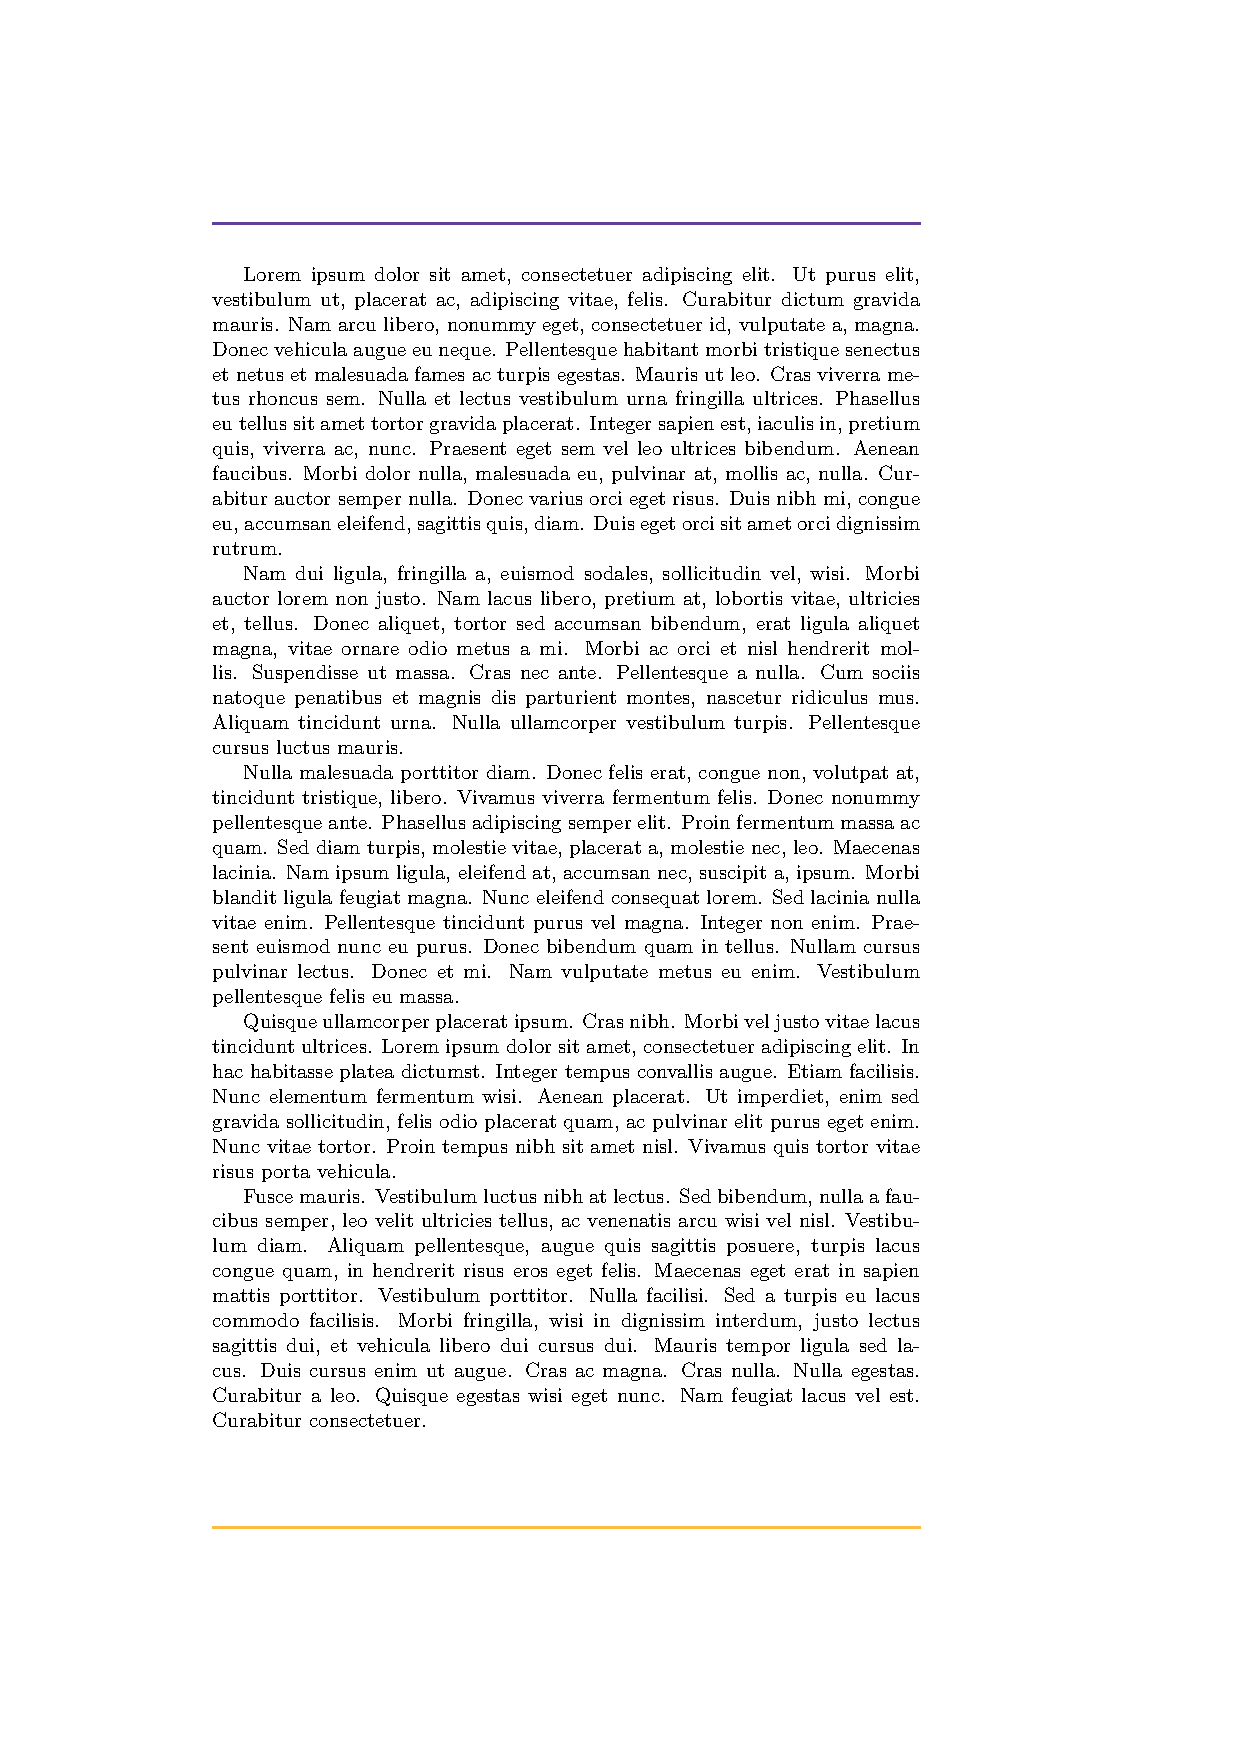
\includegraphics[frame,width=\linewidth]{demo-rule}
    \end{column}
  \end{columns}
\end{frame}

\begin{frame}[fragile]{\texttt{moresimple} Rules}
  \begin{columns}
    \begin{column}{0.6\textwidth}
      \begin{latexcode}
        % \usepackage[dvipsnames]{xcolor}
        \makepagestyle{moresimple}
        \makeevenhead{moresimple}{}{Jaeho Lee}{}
        \makeoddhead{moresimple}{}{Jaeho Lee}{}
        \makeevenfoot{moresimple}{\thepage}{}{}
        \makeoddfoot{moresimple}{}{}{\thepage}

        \makeheadrule{moresimple}{\textwidth}{1pt}
        \makeheadfootruleprefix{moresimple}|\linebreak|{\color{WildStrawberry}}{}
      \end{latexcode}
    \end{column}

    \begin{column}{0.4\textwidth}
      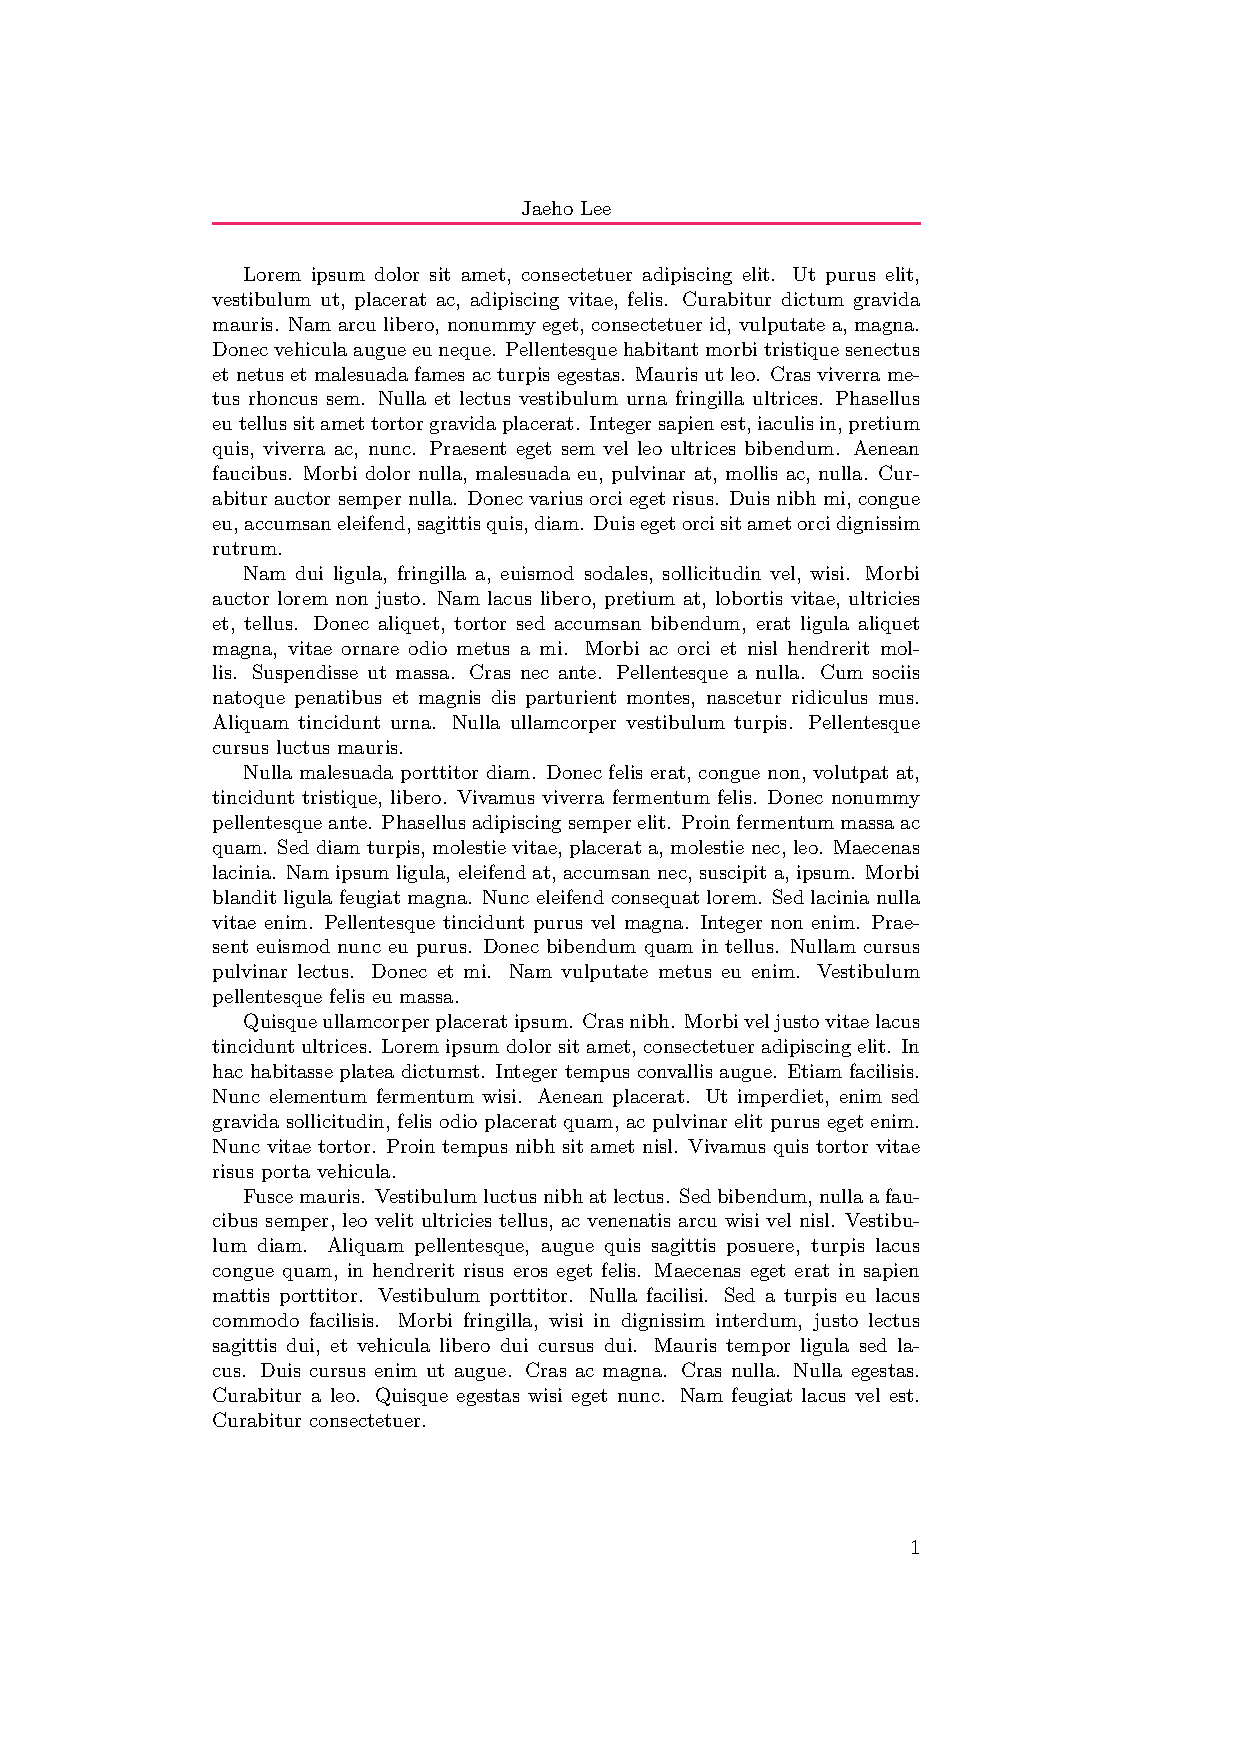
\includegraphics[frame,width=\linewidth]{moresimple-rule}
    \end{column}
  \end{columns}
\end{frame}


\section{\texttt{\textbackslash makerunningwidth}}

\begin{frame}{Rules}
  \begin{block}{The Memoir Class User Guide --- Page 110}
    The macro \ltxverb/\makerunningwidth/ sets the widths of the $⟨style⟩$
    pagestyle headers and footers.
    The header width is set to $⟨headwidth⟩$.
    If the optional $⟨footwidth⟩$ is present, then the footer
    width is set to that, otherwise to $⟨headwidth⟩$.
    The header width is stored as the length \ltxverb/\styleheadrunwidth/
    and the footer width as \ltxverb/\stylefootrunwidth/.
    The \ltxverb/\makepagestyle/ initialises the widths to be the textwidth,
    so the macro need only be used if some other width is desired.
    The length \ltxverb/\headwidth/ is provided as a (scratch) length that may
    be used for headers or footers, or any other purpose.
  \end{block}
\end{frame}

\begin{frame}[fragile]{\texttt{moresimple} Rules}
  \begin{columns}
    \begin{column}{0.6\textwidth}
      \begin{latexcode}
        \setstocksize{260mm}{190mm}
        \settrimmedsize{\stockheight}{\stockwidth}{*}
        \settrims{0pt}{0pt}
        \setlrmarginsandblock{30mm}{*}{1.618}
        \checkandfixthelayout

        % ...

        \ExplSyntaxOn
        \dim_set:Nn \headwidth { \textwidth + \marginparsep + \marginparwidth }
        \ExplSyntaxOff

        \makeheadrule{moresimple}{\headwidth}{1pt}
        \makeheadfootruleprefix{moresimple}|\linebreak|{\color{WildStrawberry}}{}
        \makerunningwidth{moresimple}{\headwidth}
        \makeheadposition{moresimple}{flushright}|\linebreak|{flushleft}{flushright}{flushleft}
      \end{latexcode}
    \end{column}

    \begin{column}{0.4\textwidth}
      \begin{overprint}
        \onslide<1>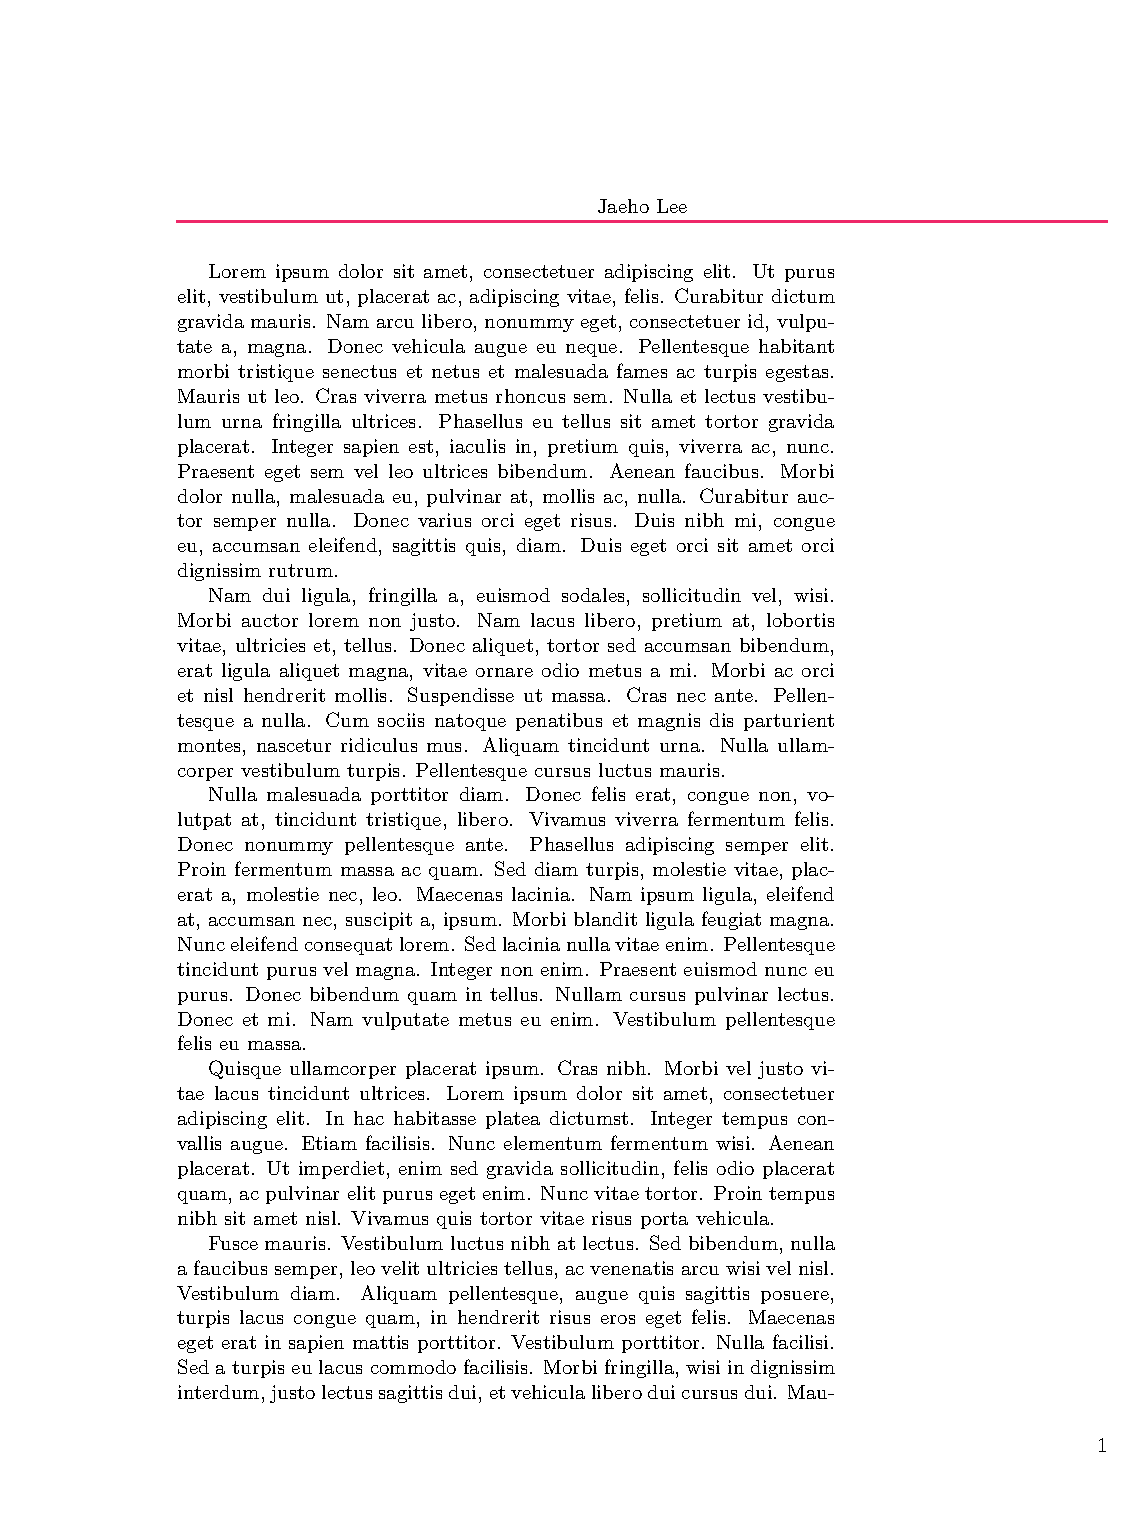
\includegraphics[frame,width=\linewidth]{moresimple-rw-1}
        \onslide<2>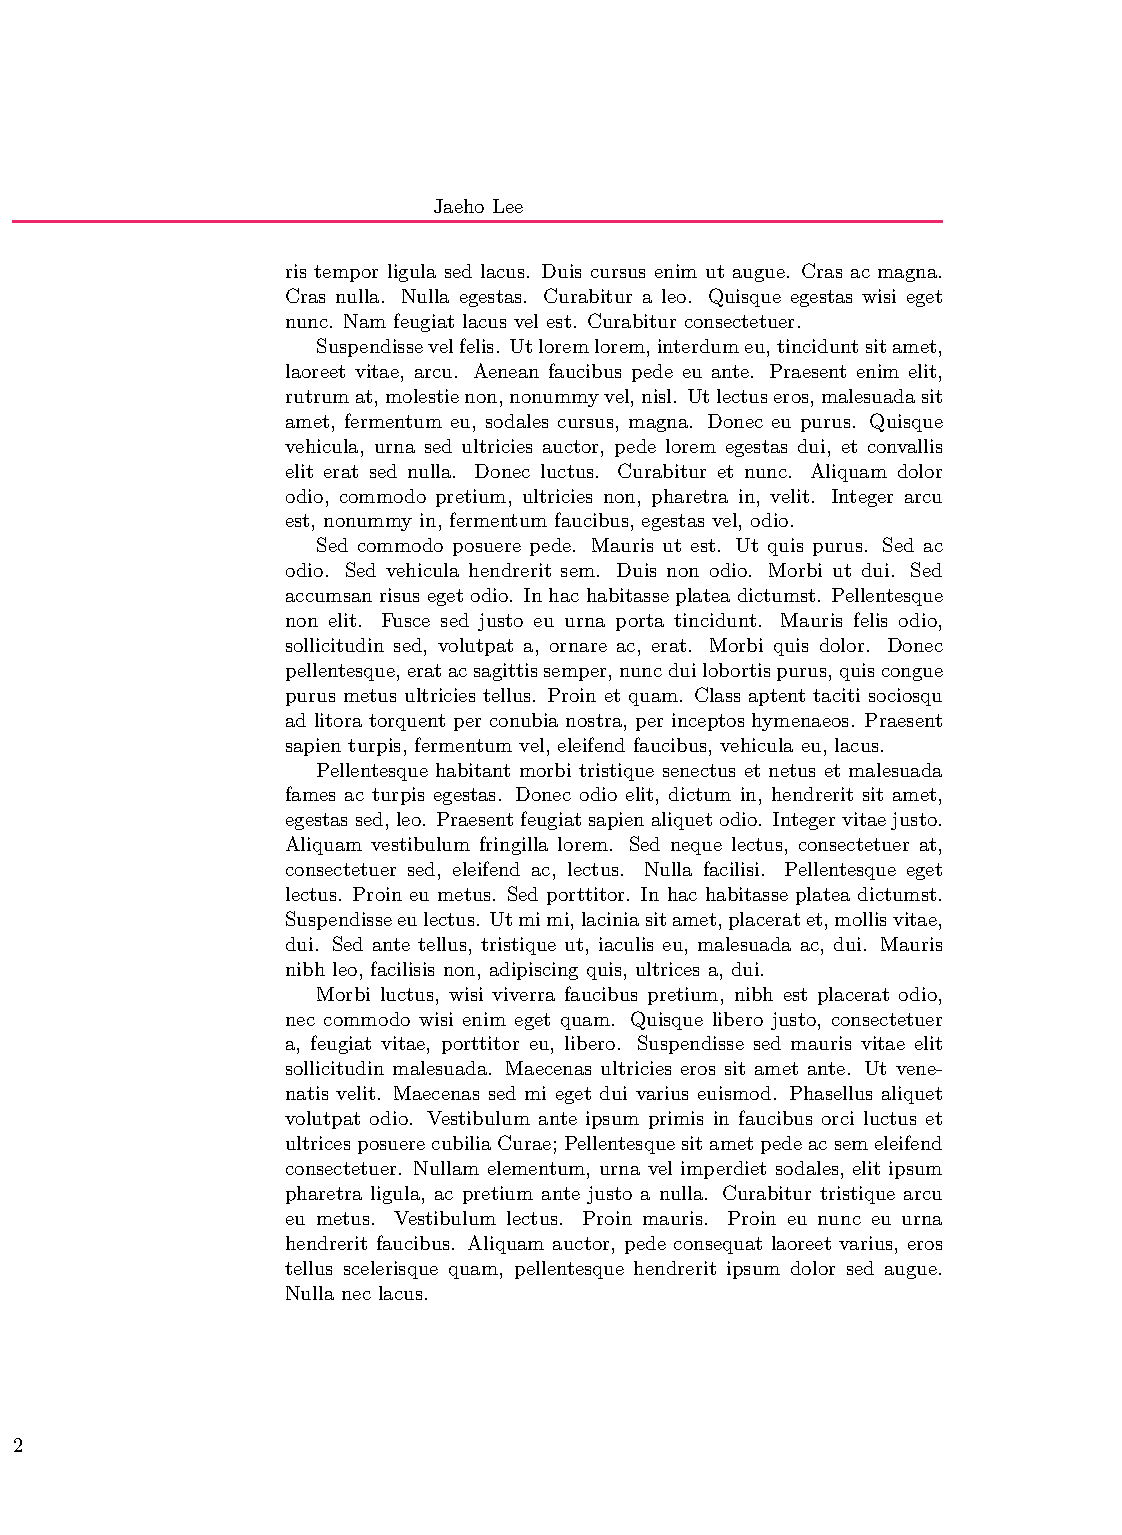
\includegraphics[frame,width=\linewidth]{moresimple-rw-2}
      \end{overprint}
    \end{column}
  \end{columns}
\end{frame}


\section{\texttt{\textbackslash makeheadposition}}

\begin{frame}[fragile]{\texttt{\textbackslash makeheadposition}}
  \begin{columns}
    \begin{column}{0.6\textwidth}
      \begin{latexcode}
        \ExplSyntaxOn
        \dim_set:Nn \headwidth { \textwidth + \marginparsep + \marginparwidth }
        \ExplSyntaxOff

        \makerunningwidth{demo}{\headwidth}
        \makeheadrule{demo}{\headwidth}{1pt}
        \makefootrule{demo}{\headwidth}{1pt}|\linebreak|{\footruleskip}
        \makeheadfootruleprefix{demo}|\linebreak|{\color{RoyalPurple}}{\color{Dandelion}}
        \makeheadposition{demo}{flushright}|\linebreak|{flushright}{center}{flushleft}
      \end{latexcode}
    \end{column}

    \begin{column}{0.4\textwidth}
      \begin{overprint}
        \onslide<1>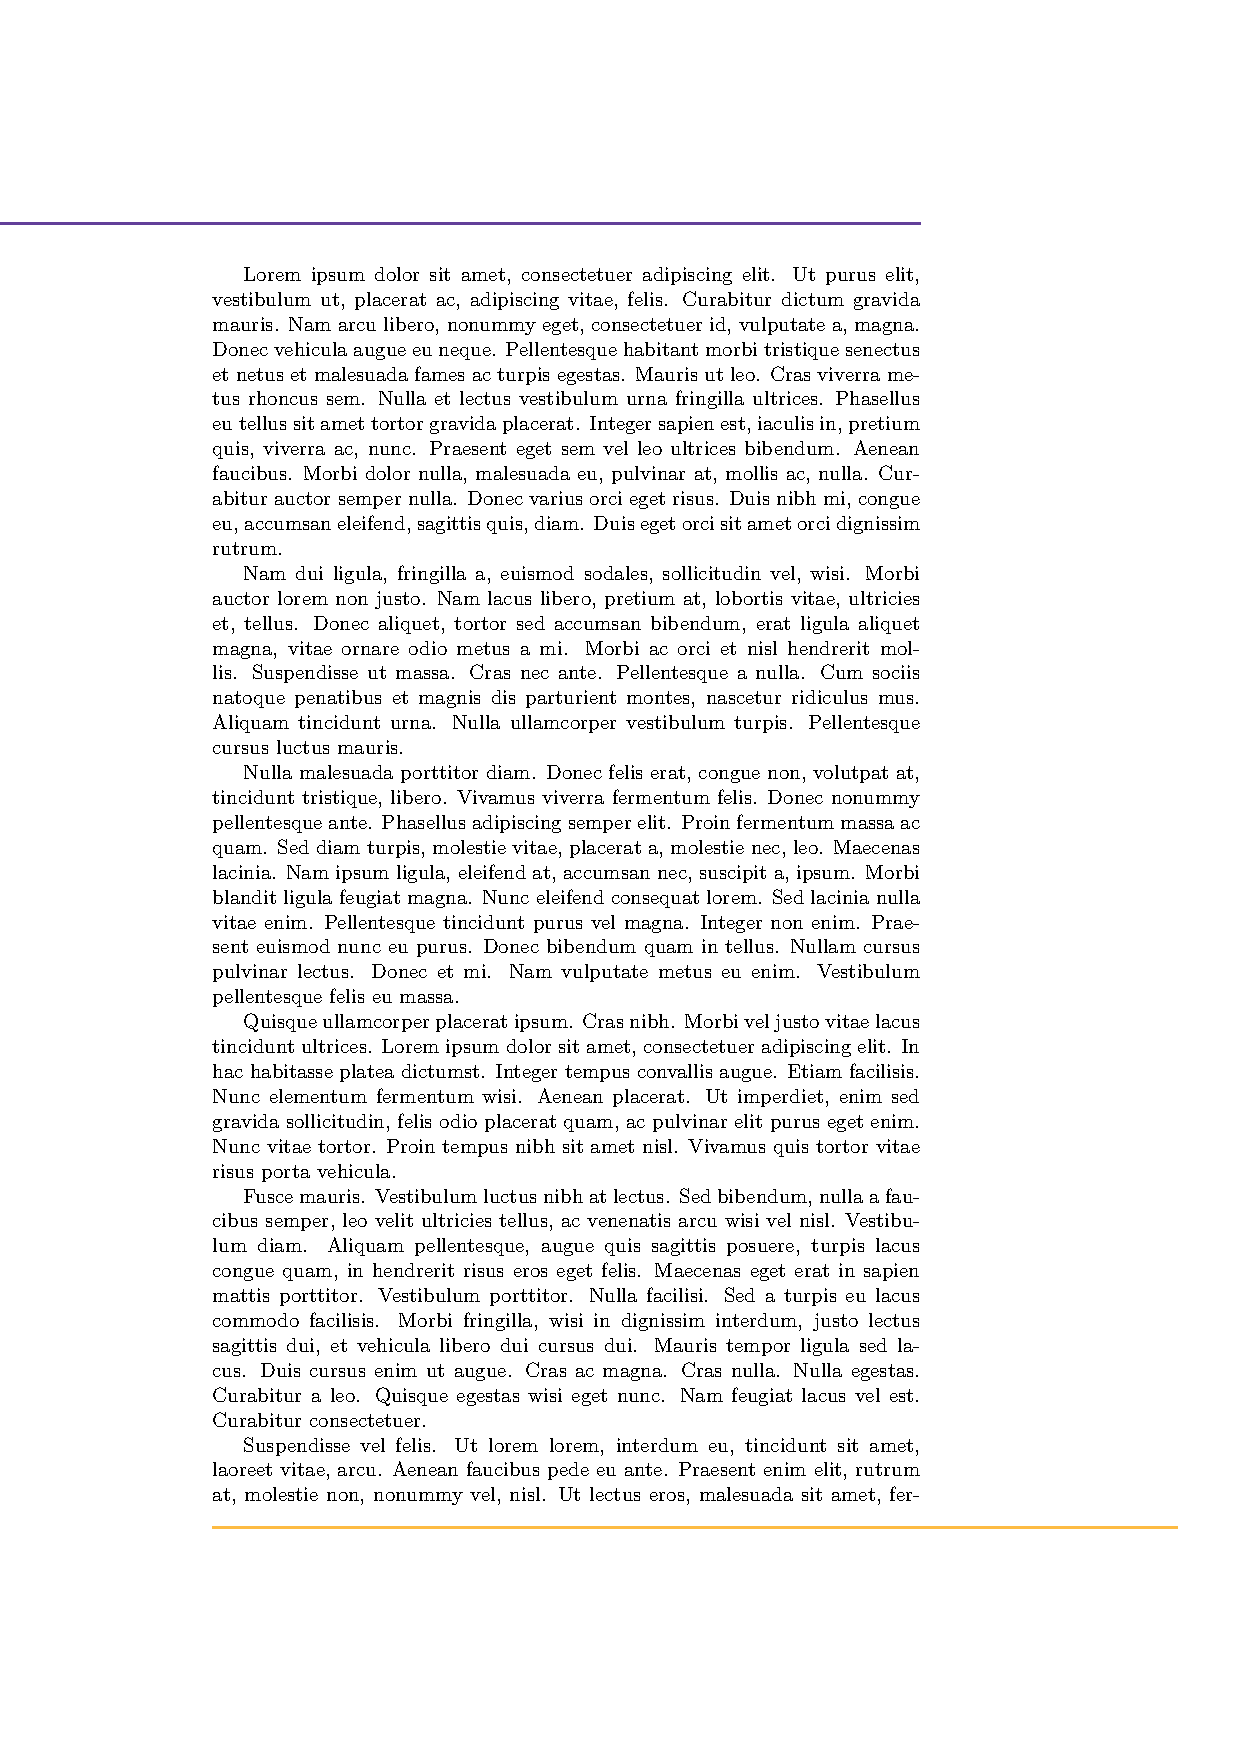
\includegraphics[frame,width=\linewidth]{demo-hp-1}
        \onslide<2>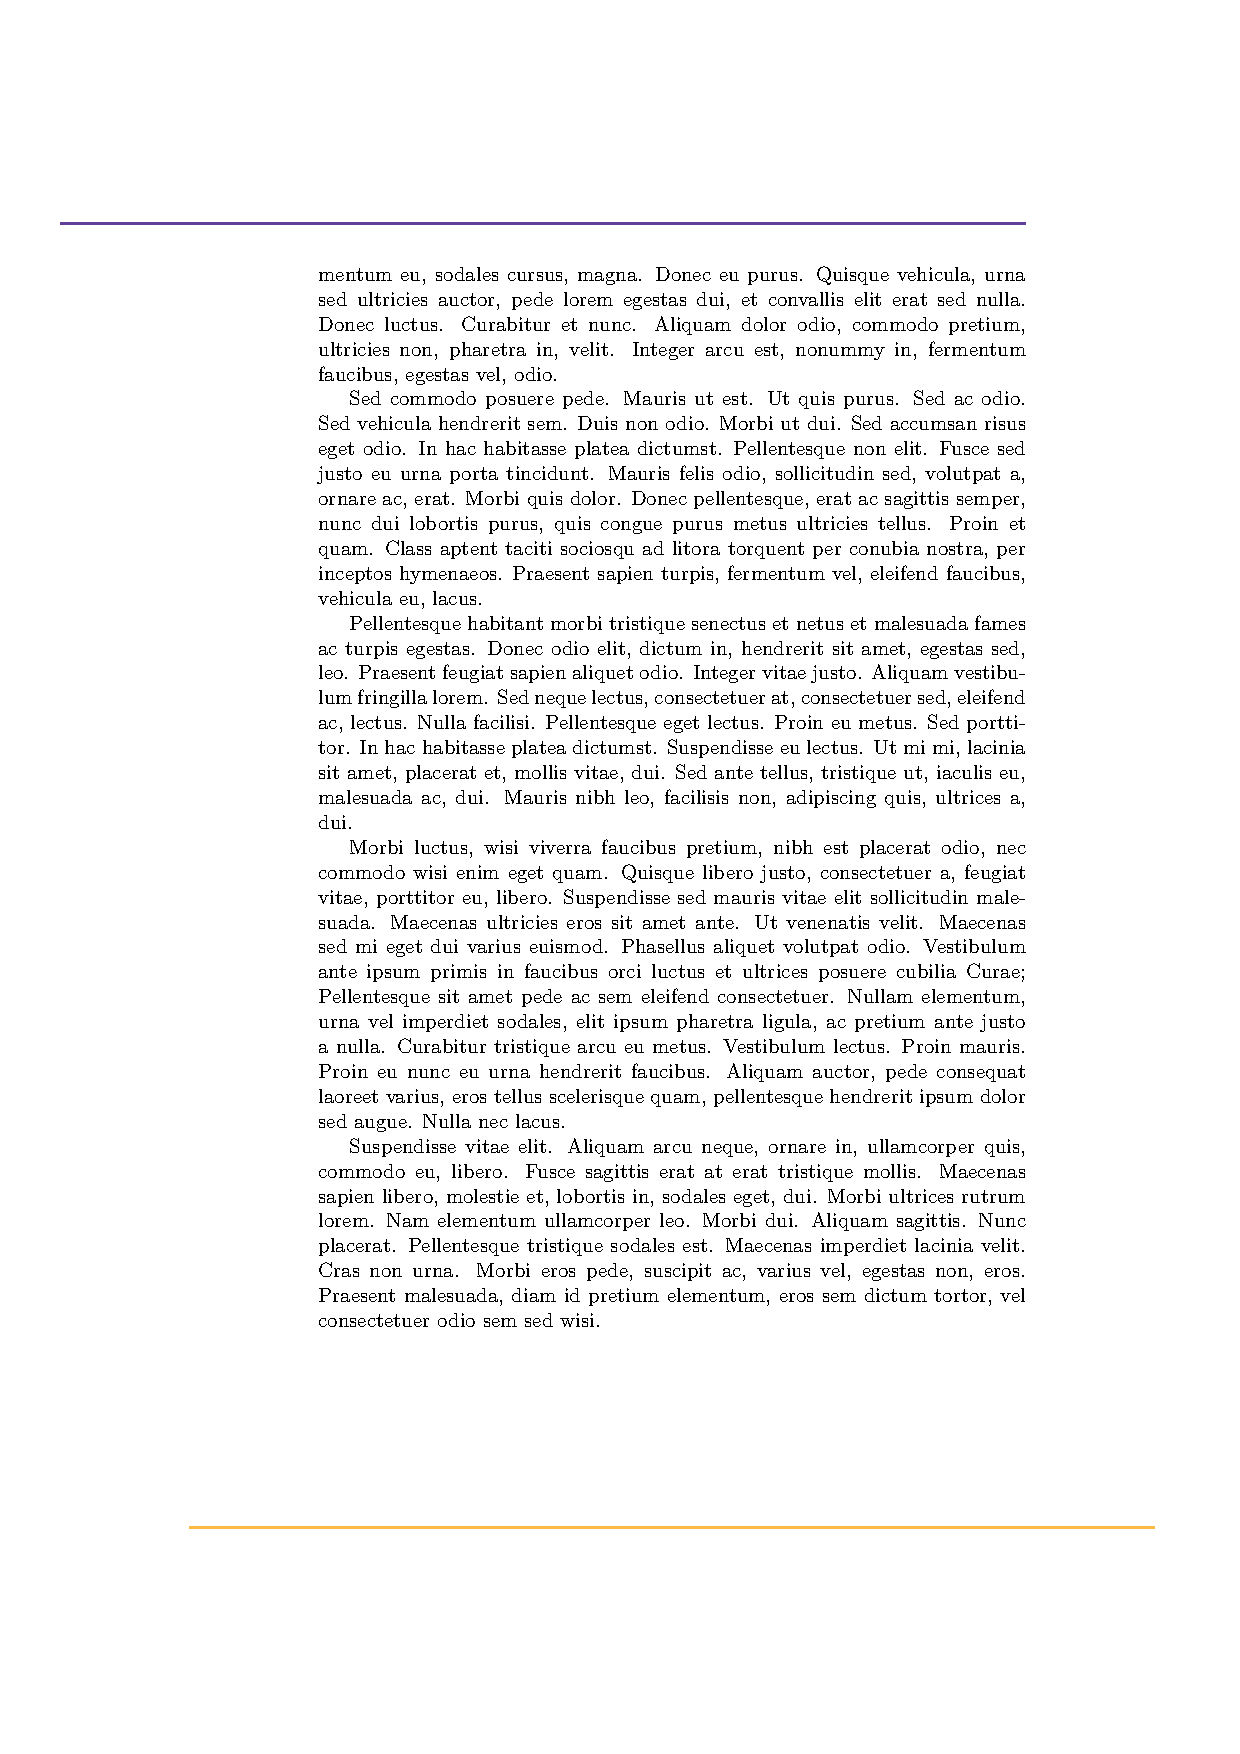
\includegraphics[frame,width=\linewidth]{demo-hp-2}
      \end{overprint}
    \end{column}
  \end{columns}
\end{frame}
\end{document}
